\chapter{Design}

\begin{longtabu} to \linewidth{@{}l l l X[j]@{}}
    Version &    Dato &    Ansvarlig &    Beskrivelse\\[-1ex]
    \midrule
    
\label{version_Systemark}
\end{longtabu}

\section{Indledning}

  
\section{Hardware arkitektur}
I følgende afsnit beskrives hvordan blodtryksmåler systemet og nogle af dets delkomponenter er opbygget.
\\
\begin{figure}[h]
	\centering
	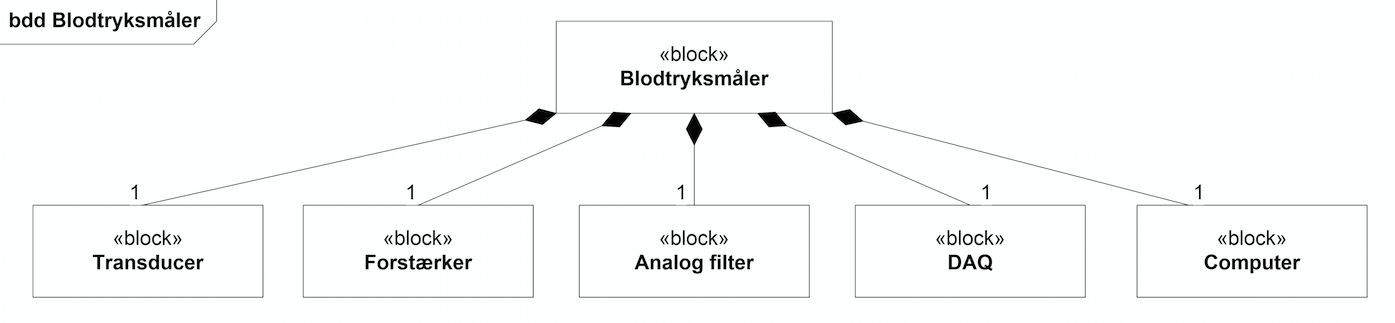
\includegraphics[width=1\textwidth]{Figurer/BDD}
	\caption{Blokdiagram for blodtryksmåler systemet.}\label{labelpic}
\end{figure}
\\Ud af blokdiagrammet kan man se at blodtryksmåler systemet består af en transducer, en forstærker, et analogt filter, en DAQ og en computer.
\\
\begin{figure}[h]
	\centering
	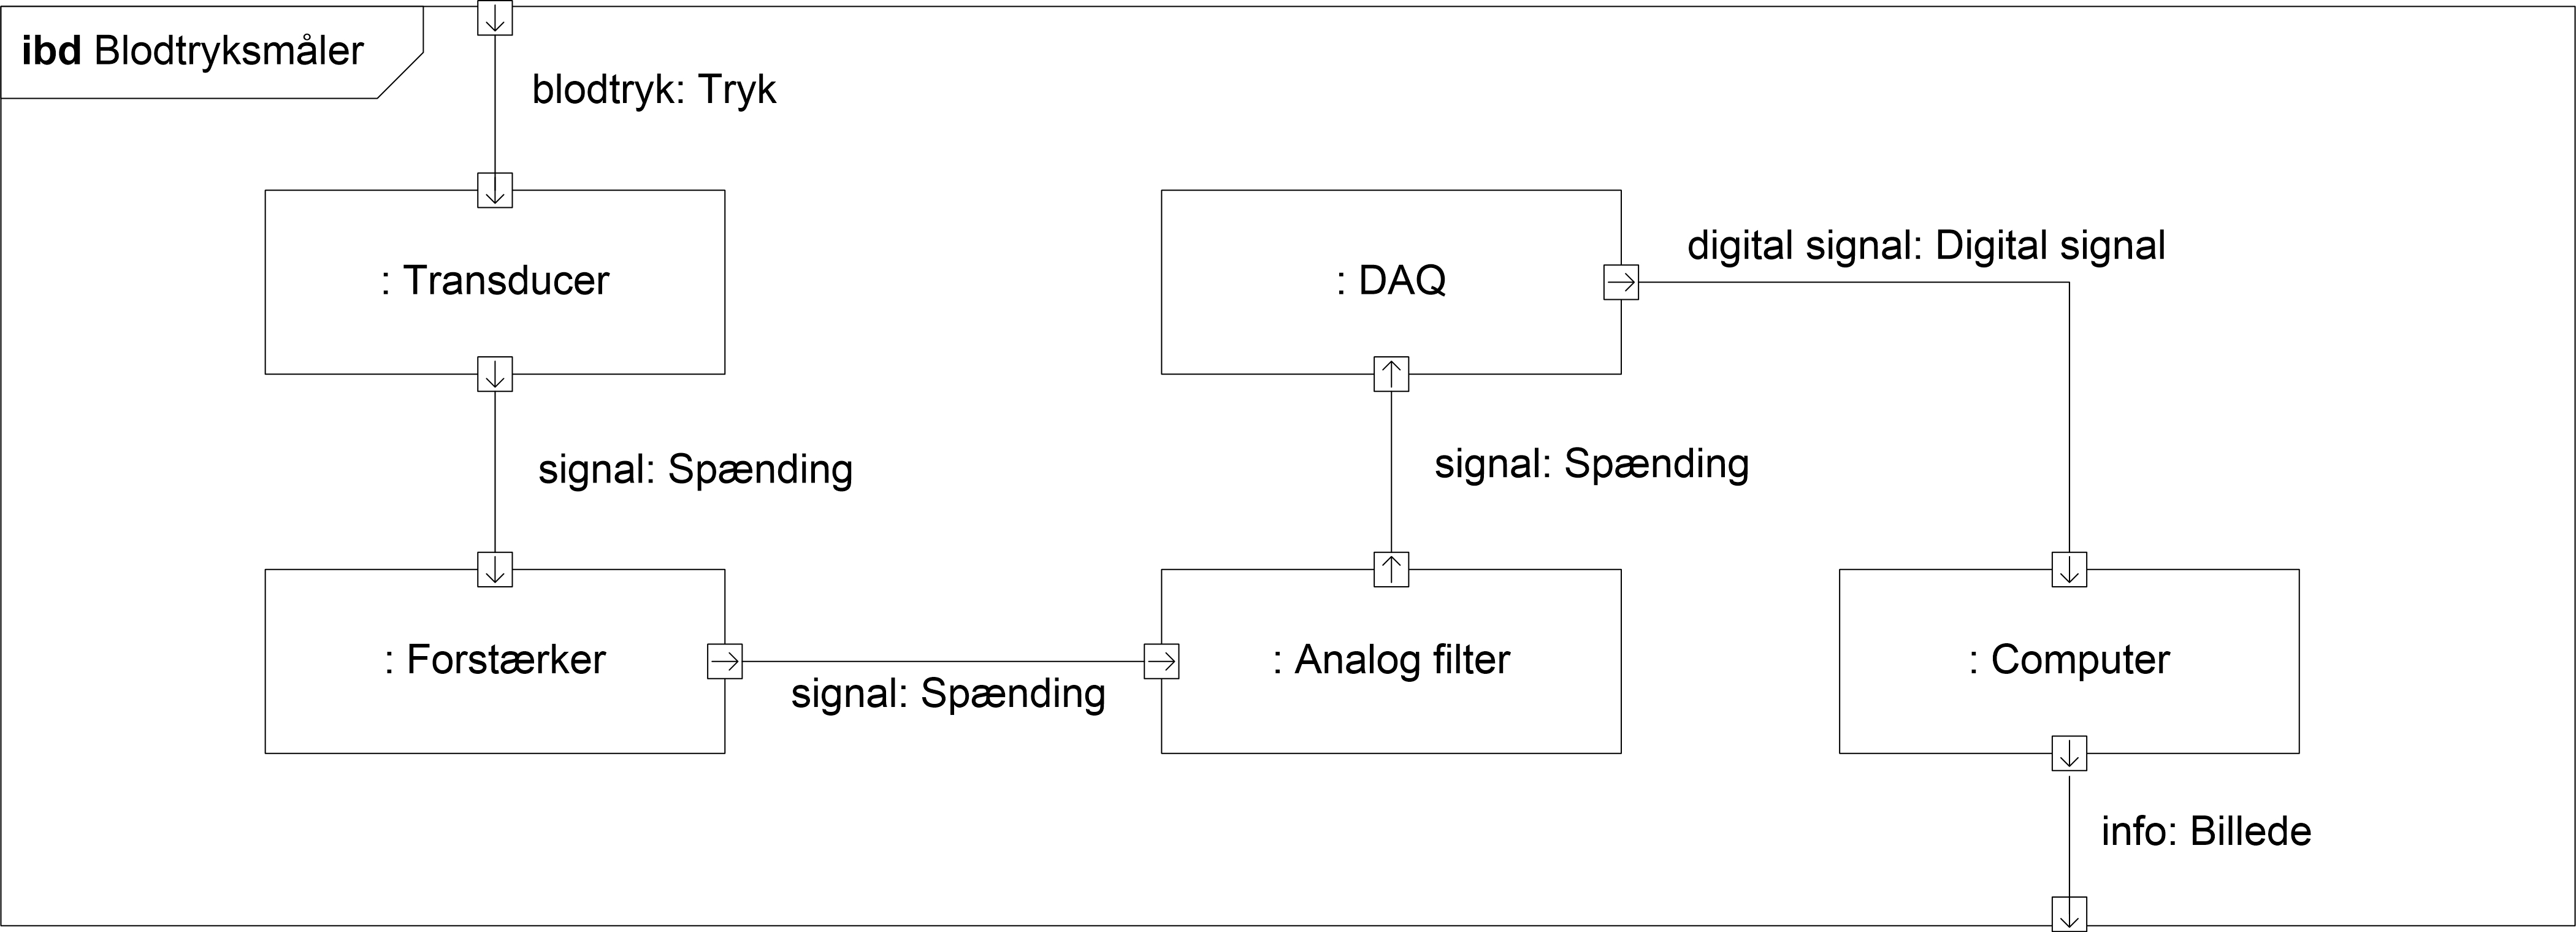
\includegraphics[width=1\textwidth]{Figurer/IBD}
	\caption{Internt blok diagram for blodtryksmåler systemet.}\label{labelpic}
\end{figure}
\\Ud af det interne blok diagram kan ses det at blodtrykket i form af det målte tryk kommer ind i transduceren. Transduceren som omformer det målte tryk til et spændingssignal, sender signalet vidre til forstærkeren. Fra forstærkeren sendes signalet over i det analoge filter og derfra ind i DAQ'en. Endeligt sendes det digitale signal fra DAQ'en over i en computer, der fortolker signalet som et billede, der vises til omverdenen.


\subsection{Design af forstærker}
Forstærkeren er designet med tanke på, at det er meget små spændinger der arbejdes med. Grundet dette, er en almindelig operationsforstærker fravalgt, da dens reelle indgangsimpedans er for lille. En Instrumentationsforstærkers indgangsimpedans i den virkelige verden, er højere, og den kan dermed opfange meget små signaler så som blodtryk.\\
Vejleder rådede herefter til at projektgruppen brugte instrumentationsforstærkeren INA114. Forstærkerens design kan ses på figur X.\\ 
\begin{figure}[h]
	\centering
	\includegraphics[width=1\textwidth]{Figurer/Forstærker}
	\caption{Der overordnede design af forstærkeren.}\label{labelpic}
\end{figure}
*Rgain* er modstanden, som bestemmer, hvor meget forstærkning, instrumentationsforstærkeren skal give og *Rload* er den belastning, der kommer efter kredsløbet. I dette tilfælde, er det, det analoge filter. For at finde *Rgain’s* størrelse, kræver det, at der vides, hvor meget forstærkning der er brug for. Dette findes, ved at bestemme den maksimale spænding, som transduceren kan give, i en blodtrykssituation. Dette regnestykke kan ses realiseret i ligning x.\\
\begin{figure}[h]
	\centering
	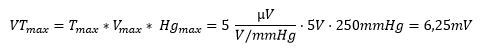
\includegraphics[width=1\textwidth]{Figurer/LigningSara}
\end{figure}



\subsection{Grænseflader}

\section{Software arkitektur}


\subsubsection{Trelagsmodellen}

\subsection{GUI}

\subsection{UML klassediagram}


\subsection{Appliktationsmodel}
 

\subsubsection{Domænemodel}

\subsubsection{Sekvensdiagram}

\subsubsection{Opdateret Klassediagram}

\section{Software implementering}
 
\subsection{Visning af EKG-signal}

\subsection{Analyse}

\subsection{Testprogram}

\subsection{Lagring i database} 

\subsubsection{Offentlig database}

\subsubsection{Privat database}







